\section{Concept}

This section illustrates the concrete idea that we have now synthesized from our general suggestions.
It is no way complete or final.
As most of these concepts are based on the location sharing, we propose to implement the location sharing first and then expand the other concepts on top of that.

\subsection{Location Sharing}
\label{location_sharing}
Location Sharing is the base service required for further development of the MIND system.
The idea is that people in an enhanced office environment can be tracked using public displays placed the offices.
So looking at a public display one can see the current location of every other office member.
A sketch of such a display is shown in figure \ref{fig:location_sharing}.
Office rooms are drawn as an floor plan and colored similarly to their assigned office members.
The members themselves are drawn in unique colors extended with a photo or sketch to make them easily identifiable.

\begin{figure}
	\centering
	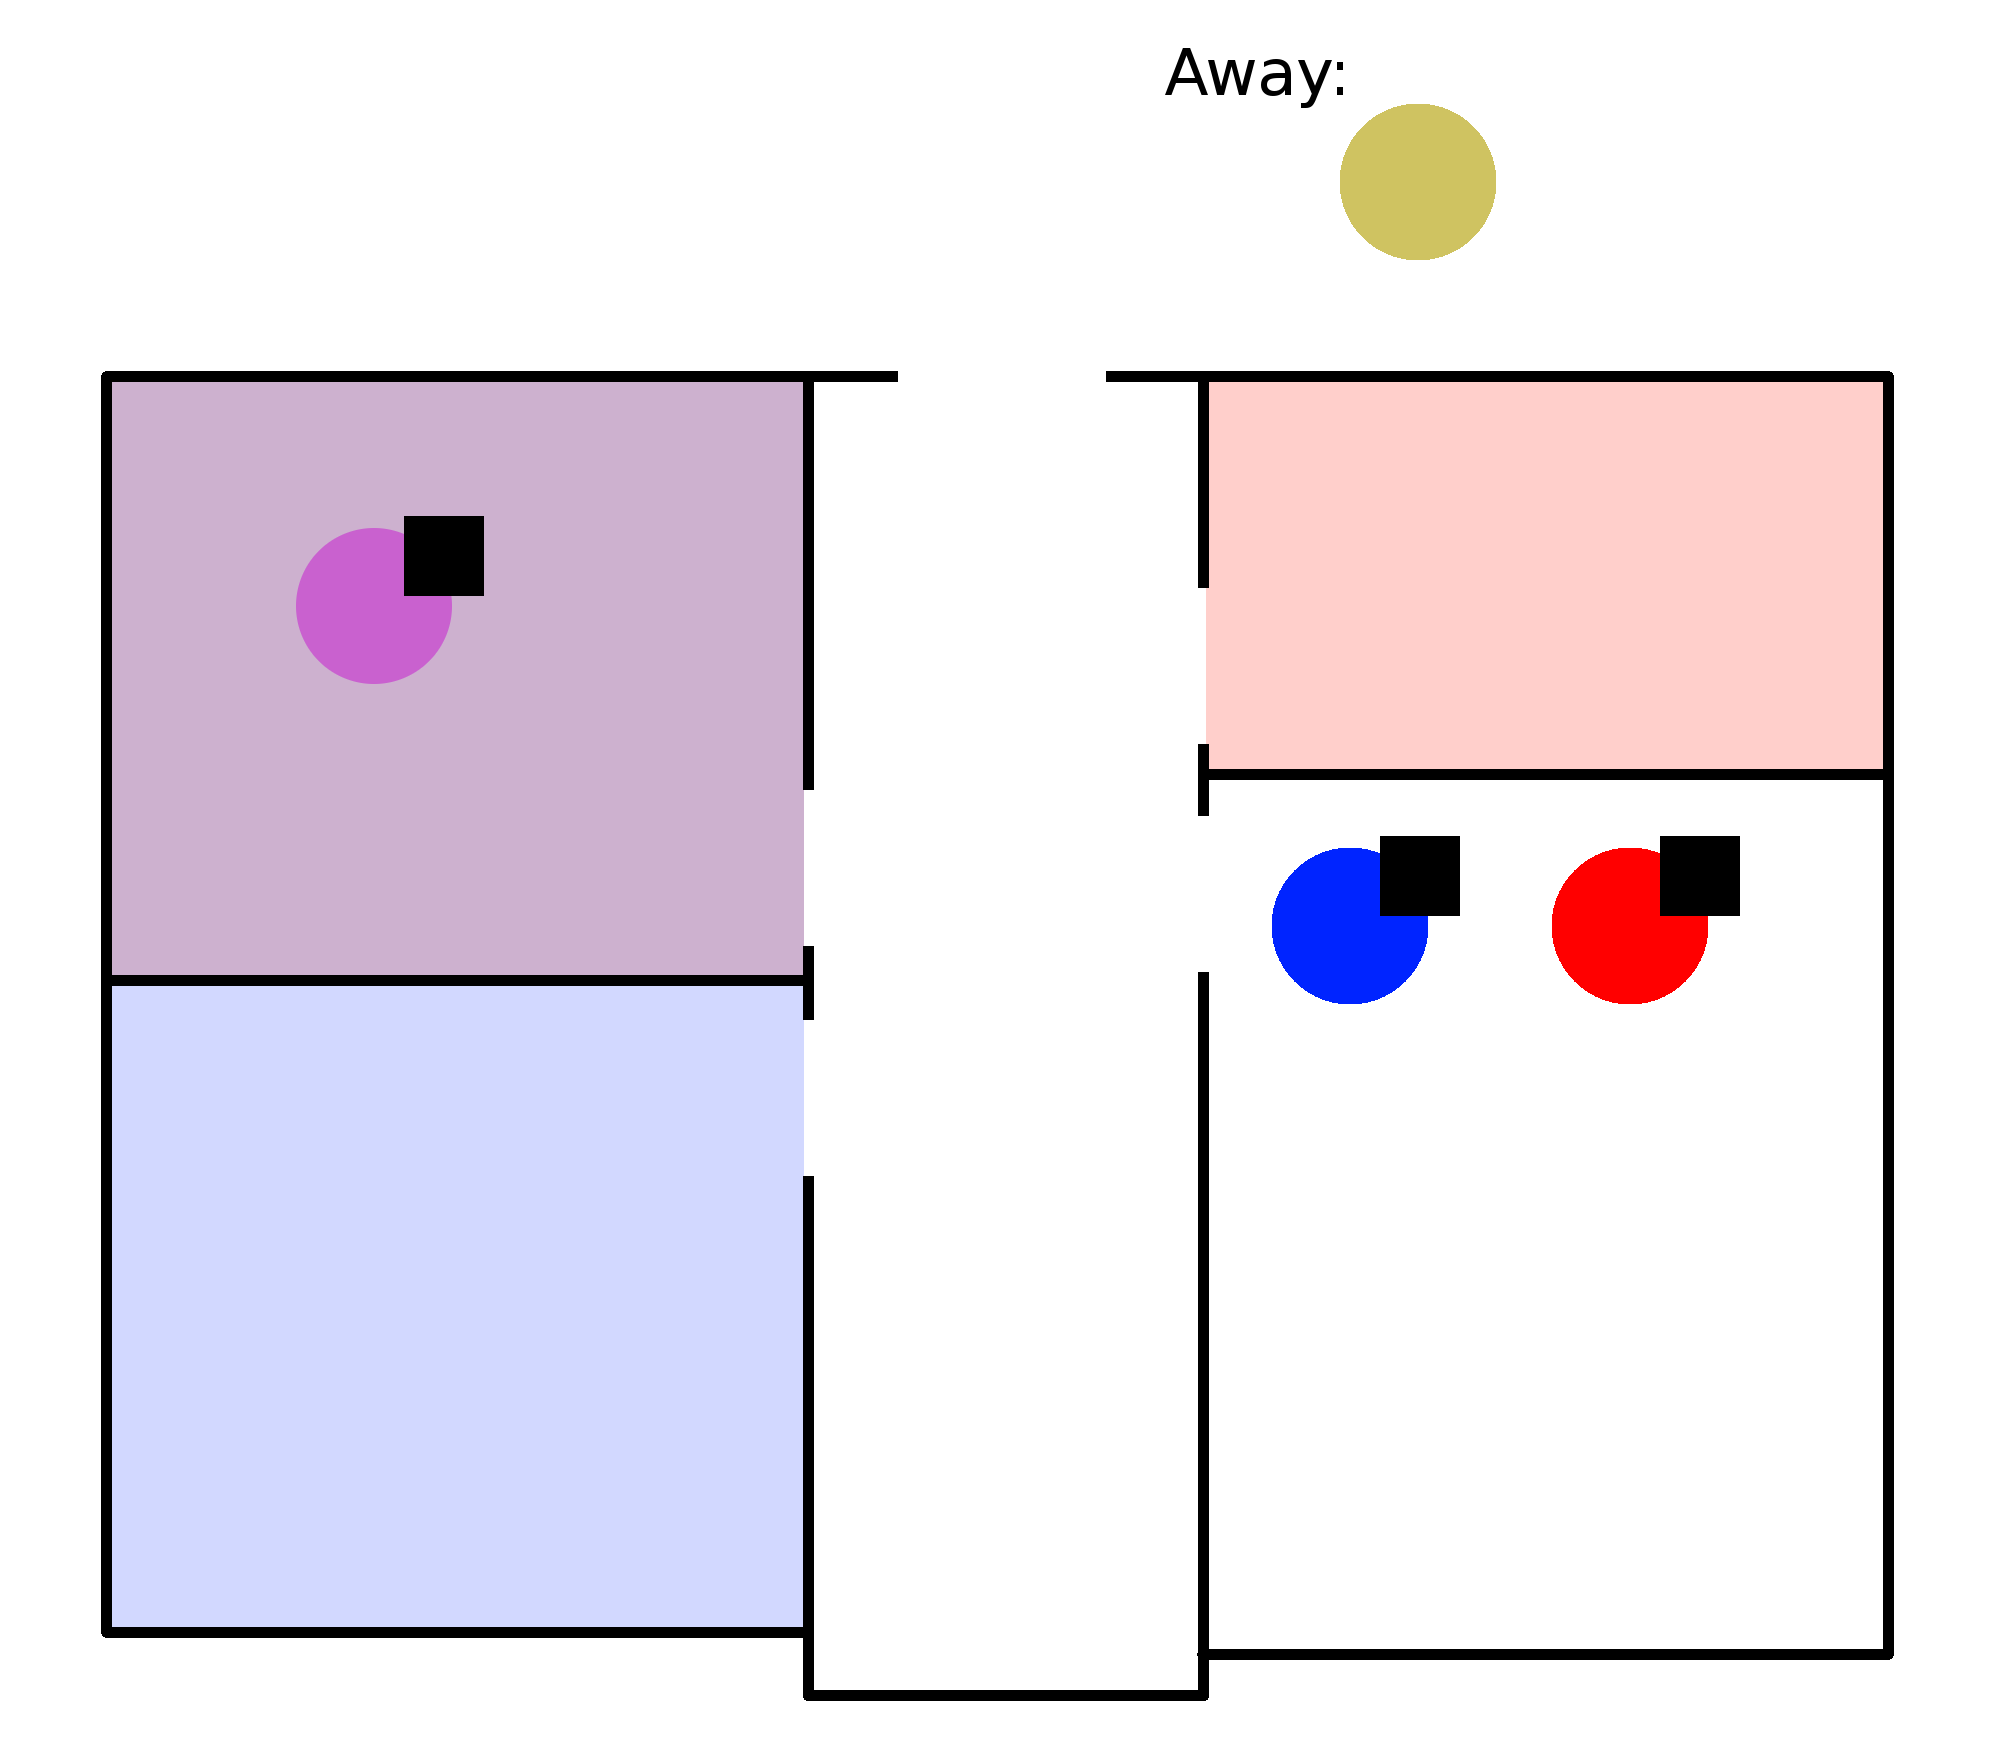
\includegraphics[width=\linewidth]{img/location_sharing}
	\caption[Location Sharing]{Location Sharing}
	\label{fig:location_sharing}
\end{figure}

The tracking is done using light sensors at doors reacting to people entering and leaving an office.
Then using wifi fingerprinting of the member's mobile device his location is determined.

Since the public display is placed within an office room, repeating changes on the screen my interrupt members working.
As consequence the display is dimmed when none is looking at it and changes are made using very smooth transitions.
Looking at the screen, the display lights up and its update frequency is increased.
This behavior is achieved using simple head tracking via camera and computer vision.

Concerning privacy not every member wants to be tracked all the time.
Also it must be possible to tell others not to be disturbed.
Therefore every member owns a configurable personal profile controlling his privacy wishes.
It allows setting different visibility stages such as hiding oneself from the system,
Showing one's general availability and his location.
The later two modes allow further adjustments such as setting 'Do not disturb'.
In any mode it is also possible to set messages such as 'currently in mensa' to notify other members of ones location when not in office.
Also the door can be used as input to control these modes.
An open door could represent availability and a closed unavailability or that the member is busy.

A web based administration interface is used to manage member-office associations.

As extension we propose to add a public display in front of the office to allow external persons such as students see which office member is currently available.
The setting if a student may see a persons availability is configured by each member individually in his privacy profile.



\subsection{Video Sharing}

The idea behind Video Streaming is that a person can call a room 
(for example the conference room) or a single person (the person’s office or a room where the person is currently in).
A Location Service can provide the current location of the person.
Assumed person A wants to start a video conference with person B. person A only sees a pixelated picture of person B. Person B sees Person A clearly. Now person B can accept the request with a gesture or an touch interaction (for example wipe to clear the view) or reject the request (see figure \ref{video_sharing_pic}).
\begin{figure}
	\centering
	\includegraphics[width=\linewidth]{img/videochat.png}
	\caption[Video Sharing]{Video Sharing - wipe to clear the view}
	\label{video_sharing_pic}
\end{figure}
To keep interruptibility small the called person only sees a pixelated picture or a frozen window (no movements). Besides, a person can configure intensity of the display’s brightness and other settings. 
To protect privacy the user can change his status from available to limited available (for example available to certain people or available in certain time slots). He also can configure that he doesn't want to be interrupted by whatever is going on. So the interruptibility is kept small too. To put this approach into practice we work with Raspberry Pis and an open source Video Streaming. It has to be checked whether the performance of the Raspberry Pis is suffice.

\subsection{Screencast Sharing}

The idea behind screen sharing is to provide a platform for displaying content from a personal device, such as a smartphone or notebook, on a public display.
The user can either share her/his whole screen or draw a bounding box, encompassing the to be shared content.
The purpose of sharing is solely to display the content, not to make the displayed information accessible e.g. in the matter of downloading data.
As a consequence, a high level of privacy is concomitant with screen sharing.
A user can share a section of her/his screen either from being located in the room with the public display where the content is intended to be displayed or while being situated in another room, e.g. her/his office.

In order to initiate screen sharing, the user configures the desired content and location in the client on the private device.
Additionally, combining screen sharing with video-chat is a possibility.

\begin{figure}
	\centering
	\includegraphics[width=\linewidth]{img/screensharing.png}
	\caption[Screen Sharing]{Shared content is marked with colored frames on the public display as well as the private devices.}
	\label{screen_sharing}
\end{figure}

\subsection{Calendar Sharing}

By including the user’s calendar (e.g. Google Calendar) into a network of public displays (MIND), the functionality of the latter can be enriched.
The system may retrieve information from the calendar, such as meetings or not assigned timeslots.
For example can the system initiate conference calls or render the accessibility of the user in the system either busy or available, dependant on the calendar entries.
The effect of the calendar on the system can be adjusted by the user via a dedicated GUI.

\subsection{Data to Go}
\label{data2go}

One part of the proposed architecture would be location aware data sharing within the display network.
This is envisioned to work in two general modes, which are based on the underlying location sharing described in section \ref{location_sharing}.
The first would allow the pinning of data to a user's location, leaving its visibility set to private.
This would allow a user to take data with him when going to a colleagues' office for a meeting.
Apart from making the data available to the system, no further care would need to be taken to keep data readily available.
The second mode would allow data to be shared by sending it to a certain location, for example a meeting room.
This would make the data publicly available, primarily for that location.
Once that shared data is accessed from the location, its ownership would transfer away from its originating owner to a public ownership based on the location.

Figure \ref{data_share_sequence} shows some concepts for how the system would handle the data via the proposed modes.
Private sharing of data is also allowed by pinning data to another person.
This person then has access to the data based on their location, although ownership only transfers at a specific event that will have to be specified based on user preference and usage for download.

\begin{figure}
	\centering
	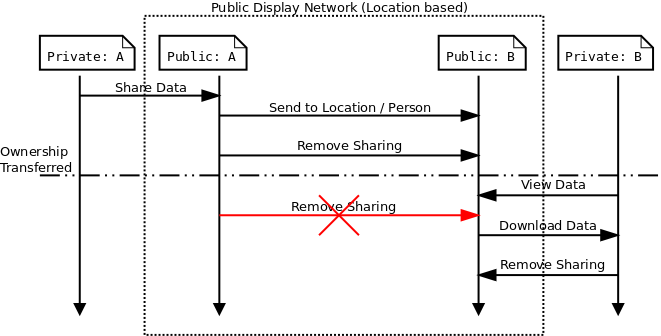
\includegraphics[width=\linewidth]{img/data_sharing.png}
	\caption[Data Sharing Sequence]{Informal sequence diagram of how data sharing might work, including some privacy and security options.}
	\label{data_share_sequence}
\end{figure}

As no data can be generated in the first iterations of the system (although such capabilities might well be added), a way to transfer data to and from the system will be required.
Such a way also makes sense from a user point of view, as the system is to be used alongside a broad range of private computers of the users.
To solve this data transfer gap, we propose a client program for a variety of devices that allows data control.
Pinning data to the user's own location (as in his private space) can be done by simply allowing the user to drag\&drop a file onto the client application, which will handle any conversion and transferring mechanism.
Similarly, retrieving data from a location or private area can be done by selecting the data via the client.
Having a client for not only desktop computers but also for smartphones would enable a broader and more comprehensive usage of the proposed service system.
